% !TEX root = ../../main.tex

\section{Physical models of adsorption}%
\label{pyg:models}

As the process of characterisation of porous materials
relies on mathematical models of adsorption, this section 
details several concepts essential to the description of the 
adsorbed phase, as well as several guest-host system archetypes.

\begin{figure}[htb]
	\centering
	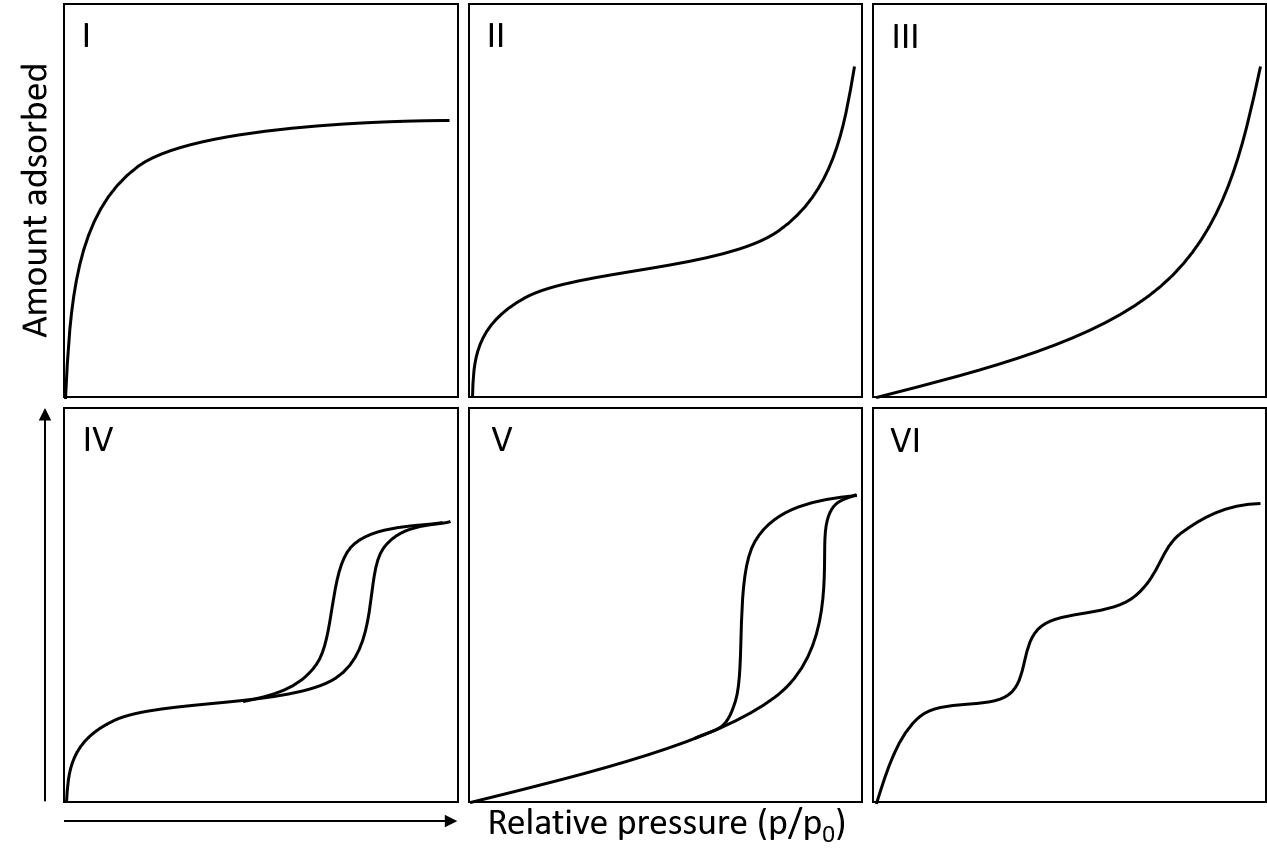
\includegraphics[width=0.8\linewidth]{iupac-isotherms}
	\caption{
		IUPAC isotherm types. 
		Adapted from \citet{rouquerolAdsorptionPowdersPorous2013}.
	}\label{pyg:fig:iupac-isotherms}
\end{figure}

Adsorption isotherms can have highly different shapes and features,
depending on the system involved. 
Much effort was put into attempting to describe and categorize
the phenomenon of adsorption, with IUPAC recommendations suggesting
six types of isotherms, as seen in \autoref{pyg:fig:iupac-isotherms}. 
While these isotherm types can be useful for fast classification, 
there is no ``one size fits all'' approach. Indeed, the only 
certain behaviour is that the amount adsorbed is zero at
the isotherm start and that the loading increases with increasing 
pressure, with the latter shown in \autoref{dut} to not be 
always true. However, through careful assumptions and a well-defined
model, the underlying mechanisms of adsorption can be understood.
Unfortunately, the plethora of isotherm features and shapes can only
be truly recreated by molecular simulation, a method which requires an
exact knowledge of the adsorbent structure and its interaction
with the guest molecules.

Nevertheless, models derived from a kinetic or thermodynamic
view of adsorption can be useful for obtaining simple parameters
which are representative of physical factors such as
guest-host interaction, surface area, pore size,
and total capacity. Thermodynamical models require a coherent
definition of the adsorbed phase, often done through the 
Gibbs surface excess approach. This description allows for an equation 
relating the bulk and adsorbed phase to be obtained, called
the Gibbs isotherm. Models which are derived from this equation include
Henry's law, the virial model and vacancy solution theory.
Adsorption can also be described from a kinetic standpoint, where
the rate of adsorption and desorption of molecules on
available sites is mathematically modelled. Equations based
on kinetics include the Langmuir model, the BET model,
the Temkin model and empirical or semi-empirical derivatives
such as the Toth, Quadratic or the Jensen-Seaton model
A page of figures for different models and how the
described isotherm varies with different values of
their parameters can be seen in
\autoref{pyg:fig:modelex}. The following section will describe
these equations, together with their assumptions and
applicability.

\begin{figure}[p]
	\centering

	\begin{subfigure}{0.3\linewidth}
		\caption{Henry}\label{pyg:fig:henryex}%
		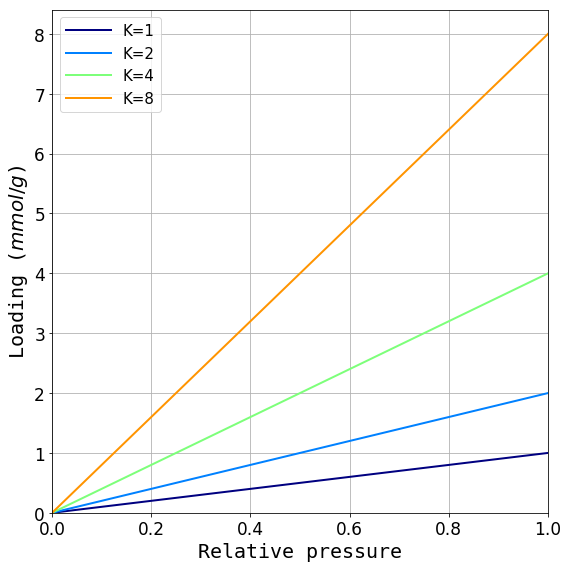
\includegraphics[width=\linewidth]{models/henry}
	\end{subfigure}%
	\begin{subfigure}{0.3\linewidth}
		\caption{Langmuir}\label{pyg:fig:langmuirex}%
		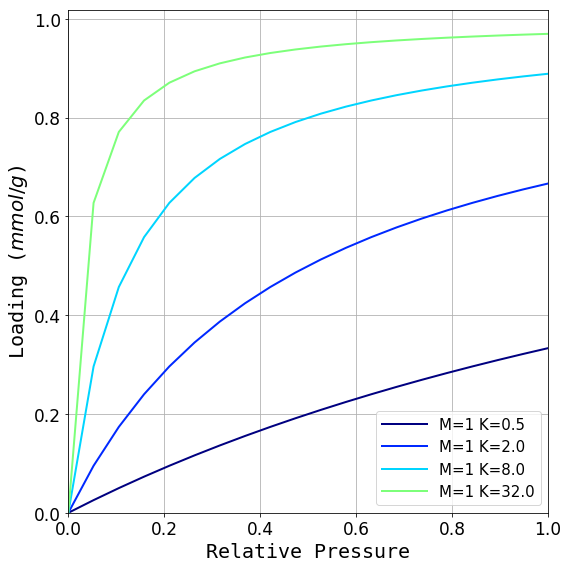
\includegraphics[width=\linewidth]{models/langmuir}
	\end{subfigure}%
	\begin{subfigure}{0.3\linewidth}
		\caption{BET}\label{pyg:fig:betex}%
		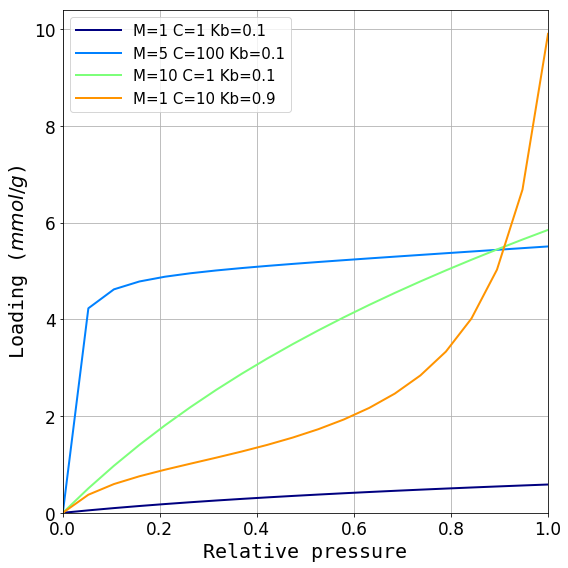
\includegraphics[width=\linewidth]{models/bet}
	\end{subfigure}%
	\\
	\begin{subfigure}{0.3\linewidth}
		\caption{Toth}\label{pyg:fig:tothex}%
		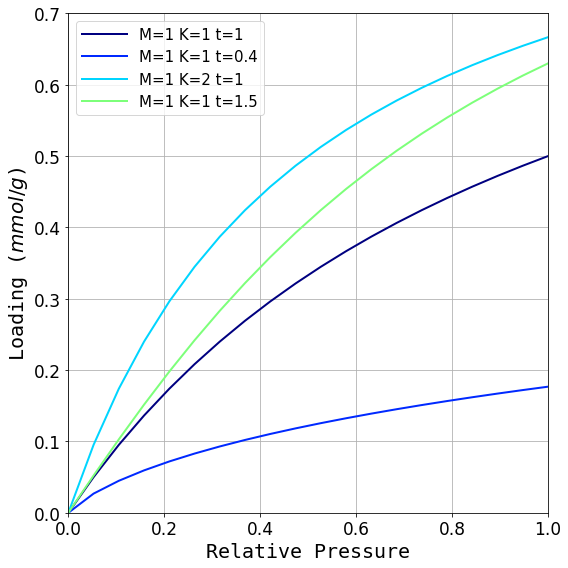
\includegraphics[width=\linewidth]{models/toth}
	\end{subfigure}%
	\begin{subfigure}{0.3\linewidth}
		\caption{Quadratic}\label{pyg:fig:quadraticex}%
		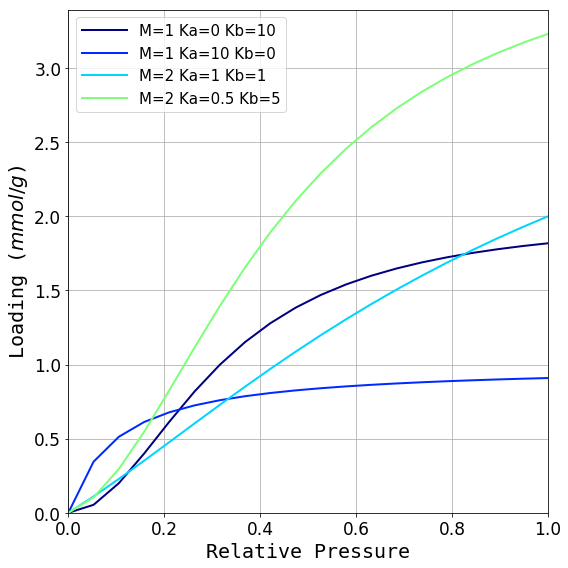
\includegraphics[width=\linewidth]{models/quadratic}
	\end{subfigure}%
	\begin{subfigure}{0.3\linewidth}
		\caption{Jensen Seaton}\label{pyg:fig:jseatonex}%
		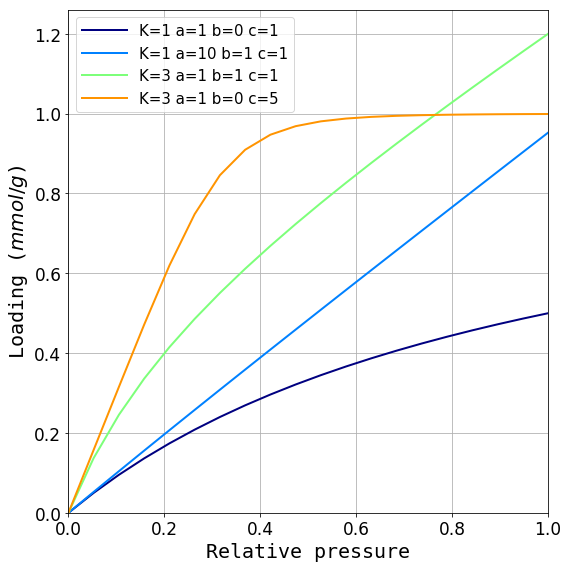
\includegraphics[width=\linewidth]{models/jseaton}
	\end{subfigure}%
	\\
	\begin{subfigure}{0.3\linewidth}
		\caption{Temkin}\label{pyg:fig:temkinex}
		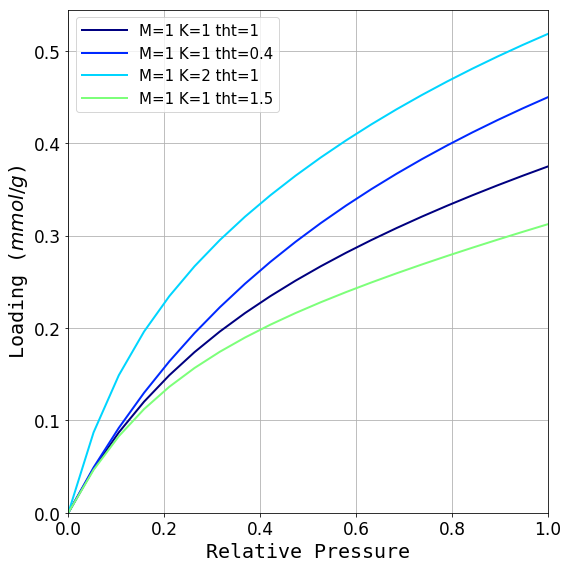
\includegraphics[width=\linewidth]{models/temkin}
	\end{subfigure}%
	\begin{subfigure}{0.3\linewidth}
		\caption{Virial}\label{pyg:fig:virialex}%
		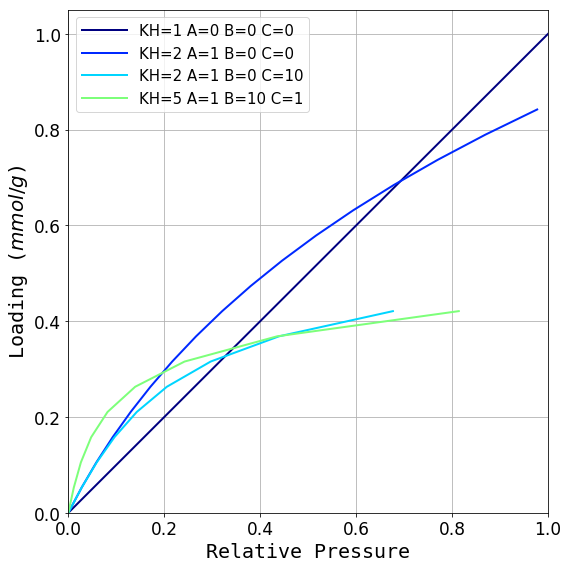
\includegraphics[width=\linewidth]{models/virial}
	\end{subfigure}%
	\begin{subfigure}{0.3\linewidth}
		\caption{W-VST}\label{pyg:fig:wsvstex}%
		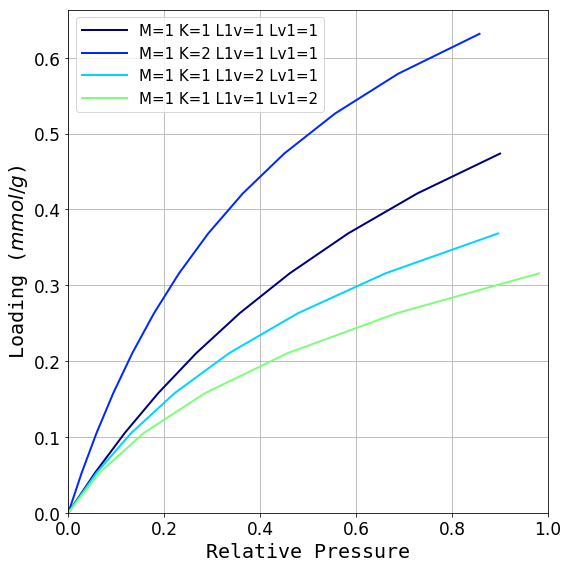
\includegraphics[width=\linewidth]{models/wvst}
	\end{subfigure}%
	\\
	\begin{subfigure}{0.3\linewidth}
		\caption{FH-VST}\label{pyg:fig:fhvstex}%
		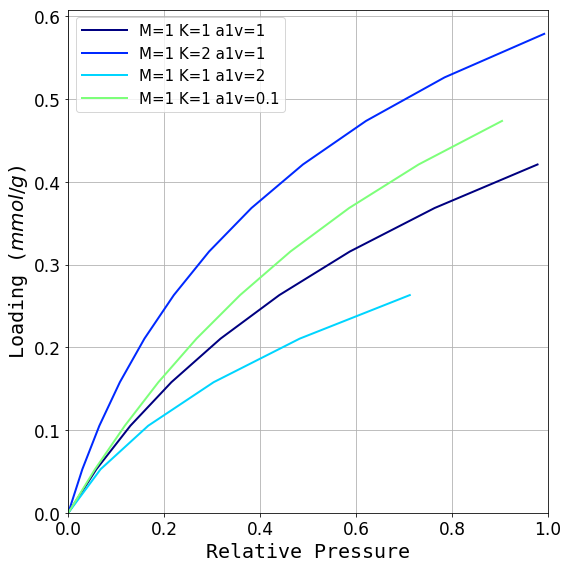
\includegraphics[width=\linewidth]{models/fhvst}
	\end{subfigure}%

	\caption{The various adsorption models
		discussed in this chapter, alongside the influence
		of their parameters on the resulting isotherm.
	}\label{pyg:fig:modelex}
\end{figure}

\subsection{The Gibbs surface excess approach}\label{pyg:models:gibbs}

A description of the adsorbed phase can be made through
expressing the change in density or concentration of fluid
from the adsorbent surface to the bulk phase. The density
has a maxima in the immediate zone close to the surface, and then
decreases until it reaches the density of the bulk fluid.
However, when defined as such, the boundary between the
two phases is difficult to pinpoint.
Therefore, in most cases it is useful to employ the concept
of the Gibbs dividing surface.

\begin{figure}[htb]
	\centering
	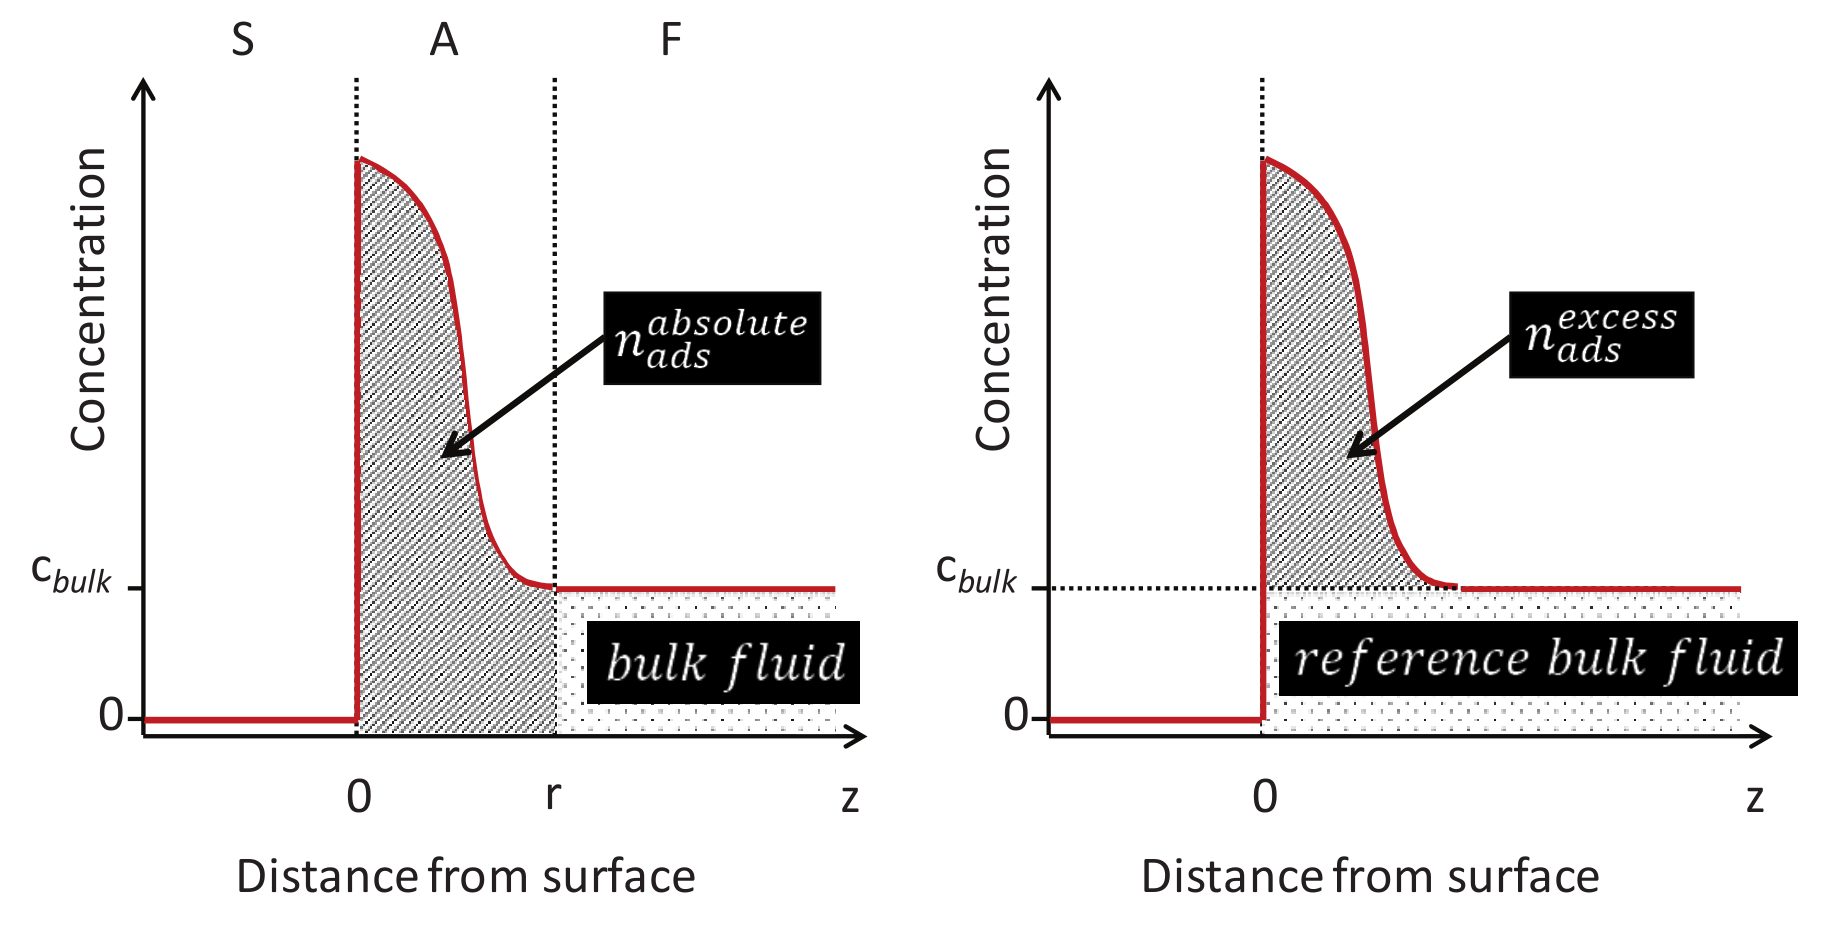
\includegraphics[width=\linewidth]{gibbs-surface}
	\caption{
		Representation of the adsorbed and bulk phases according to
		the (left) layer model and the (right) Gibbs dividing surface
		approach. Adapted from \citet{rouquerolAdsorptionPowdersPorous2013}.
	}\label{pyg:fig:gibbs-surface}
\end{figure}

This approach describes the adsorbed phase only in terms
of an \textit{excess} from the properties of the bulk phase.
As represented in \autoref{pyg:fig:gibbs-surface}, the total
amount adsorbed can be defined as:
%
\begin{equation}
	n_{ads}^{a} = A \int_0^r c\ dz
\end{equation}
%
The imaginary Gibbs dividing surface is usually envisaged parallel to
the real surface of the adsorbent and in the resulting system, the
concentration of the adsorbent in the adsorbed phase are
expressed as an excess from the concentration of the bulk fluid.
The relationship between the total amount adsorbed and the
excess amount adsorbed is then:
%
\begin{equation}\label{pyg:eqn:total-excess}
	n_{ads}^{\sigma} = n_{ads}^{a} +  c_{bulk} \cdot V_{ads}
\end{equation}

As long as the volume of the adsorbed layer \(V_{ads}\) can be
considered negligible and the concentration of adsorbate in the bulk
phase \(c_{bulk}\) is low, the total amount adsorbed and the surface
excess amount may be considered as approximately equal.
This is usually the case for experiments such as nitrogen
adsorption at \SI{77}{\kelvin}, or ambient temperature adsorption
below \SI{1}{\bar}.
At high pressures, or when the difference in concentration between
the adsorbed and the bulk phase is low, the total amount adsorbed
begins to diverge significantly from the surface excess.

In most cases, isotherms are reported in terms of excess surface 
amount. From an engineering viewpoint, this representation
is often more useful. However, any modelling and simulations of 
isotherms refers to the total amount adsorbed.
If \(n_t\) is to be calculated, a value
for the volume of the adsorbed phase and the sample is required, for a 
correction using \autoref{pyg:eqn:total-excess}.
In the case of adsorption in porous materials, the volume of the
adsorbed phase may be taken as the total pore volume. This approach
assumes that the volume enclosed by the Gibbs dividing surface is
the same as the volume of the sample, which may not be the case 
if it is determined with a blank measurement of a 
non-adsorbing gas.

Isotherm models which have a thermodynamical basis are derived
from the Gibbs equation (\autoref{pyg:eqn:gibbs}). 
The pressure and volume concepts of the bulk phase
are replaced by the 2-dimensional analogues of spreading pressure 
(\( \pi \)) and surface area.
%
\begin{equation}\label{pyg:eqn:gibbs}
	\Big(\frac{d\pi}{d\ln{p}}\Big) = \frac{n}{A} R_g T
\end{equation}
%
By substituting spreading pressure with an equation
of state for the adsorbed phase, an expression for the amount
adsorbed can be obtained as a function of bulk phase pressure.

\subsection{The Henry model}\label{pyg:models:henry}

The simplest method of describing adsorption on a
surface is Henry’s law. It assumes only interactions
with the adsorbate surface and is described by a
linear dependence of adsorbed amount with
increasing pressure.
%
\begin{equation}\label{pyg:eqn:henry}
	n_a(p) = K_H p
\end{equation}
%
It is derived from the Gibbs isotherm, by substituting a
a two dimensional analogue to the ideal gas law.
From a physical standpoint, Henry's law is unrealistic as adsorption sites
will saturate at higher pressures. However, the constant \(K_H\),
or Henry’s constant, can be thought of as a measure of the strength
of the interaction of the probe gas with the surface. At very
low concentrations of gas there is a
thermodynamic requirement for the applicability of Henry's law.
Therefore, most models reduce to \autoref{pyg:eqn:henry}
as \(\lim_{p \to 0} n(p)\).

\subsection{Langmuir and multi-site Langmuir
	model}\label{pyg:models:langmuir}

The Langmuir theory~\cite{langmuirAdsorptionGasesPlane1918},
proposed at the start of the 20th century, states that
adsorption takes place on specific sites on a surface, until
all sites are occupied.
It was originally derived from a kinetic model of gas adsorption and
is based on several assumptions.

\begin{itemize}

	\item All sites are equivalent and have the same chance of
	      being occupied.
	\item Each adsorbate molecule can occupy one adsorption site.
	\item There are no interactions between adsorbed molecules.
	\item The rates of adsorption and desorption are proportional
	      to the number of sites currently free and currently occupied,
	      respectively.
	\item Adsorption is complete when all sites are filled.

\end{itemize}

Using these assumptions we can define rates for both adsorption and
desorption. The adsorption rate (\autoref{pyg:eqn:langmuir_ads})
will be proportional to the number of sites available on the surface,
as well as the number of molecules in the gas, which is given by
pressure.
The desorption rate, on the other hand, will be proportional to the
number of occupied sites and the energy of adsorption
(\autoref{pyg:eqn:langmuir_des}).
It is also useful to define \(\theta = n_a/n_a^m\) as the fractional
surface coverage, the number of sites occupied divided by the total 
sites. At equilibrium, the rate of adsorption and the rate of
desorption are equal, therefore the two equations can be combined.
The equation can then be arranged to obtain an expression for the
loading called the Langmuir model (\autoref{pyg:eqn:langmuir}).
%
\begin{align}
	v_a                & = k_a p (1 - \theta) \label{pyg:eqn:langmuir_ads} \\
	v_d                & = k_d \theta \exp{\Big(-\frac{E_{ads}}{RT}\Big)}
	\label{pyg:eqn:langmuir_des}                                           \\
	v_a                & = v_d                                             \\
	k_a p (1 - \theta) & = k_d \theta \exp{\Big(-\frac{E_{ads}}{RT}\Big)}  \\
	n_a(p)             & = n_a^m \frac{Kp}{1+Kp} \label{pyg:eqn:langmuir}
\end{align}
%
The Langmuir constant \(K\) is the product of the individual
desorption and adsorption constants \(k_a\) and \(k_d\) and exponentially
related to the energy of adsorption \(E_{ads}\).

A common extension to the Langmuir model is to consider
the experimental isotherm to be the sum of several Langmuir-type
isotherms, each with specific maximum coverage and affinities.
The underlying assumption is that the adsorbent has several distinct
types of homogeneous adsorption sites and a Langmuir
equation is used for each. This is particularly
applicable in cases where the structure of the adsorbent
suggests that different types of sites are present,
such as in crystalline materials of variable chemistry like
zeolites and MOFs. The resulting isotherm equation becomes:
%
\begin{equation}\label{pyg:eqn:langmulti}
	n_a(p) = \sum_i n_{a,i}^m\frac{K_i p}{1+K_i p}
\end{equation}
%
In practice, only up to three adsorption sites are usually
considered.

\subsection{BET model}\label{pyg:models:bet}

Like the Langmuir model, The BET model~\cite{brunauerAdsorptionGasesMultimolecular1938}
assumes that adsorption is kinetically driven and takes place on adsorption
sites at the material surface. However, each adsorbed molecule becomes,
in itself, a secondary adsorption site, such that incremental layers
are formed. The conditions imagined by the BET model are:

\begin{itemize}
	\item The surface adsorption sites are equivalent, and therefore the
	      surface is considered homogeneous.
	\item There are no lateral interactions between adsorbed
	      molecules.
	\item The adsorption occurs in layers, with adsorbed
	      molecules acting as sites for the next layer.
	\item The energy of adsorption on subsequent layers after 
		  the initial monolayer is equal to the liquefaction energy
		  of the adsorbate.
\end{itemize}

A percentage of the surface \(\theta_x\) is occupied with
x layers. For each layer at equilibrium, the adsorption and
desorption rates must be equal.
The Langmuir model is then applied for each of layer
as shown in \autoref{pyg:tab:bet-deriv}. It is assumed
that the adsorption energy of a molecule on the second
and higher layers is just the condensation energy of the
adsorbent \(E_{i>1} = E_L\). Since it follows that
all layers beside the first have the same properties,
we can also define \(g= {k_{d_2}}{k_{a_2}} = {k_{d_3}}{k_{a_3}} =
\cdots \).

\begin{table}[h]
	\centering
	\caption{Derivation of the BET method from each adsorbed layer}%
	\label{pyg:tab:bet-deriv}
	\begin{tabular}{cc}
		\toprule
		All layers                                         & Re-arranged \\
		\midrule
		\parbox{0.4\textwidth}{\begin{align*}
				k_{a_1} p \theta_0     & = k_{d_1} \theta_1
				\exp{\Big(-\frac{E_1}{RT}\Big)}             \\
				k_{a_2} p \theta_1     & = k_{d_2} \theta_2
				\exp{\Big(-\frac{E_2}{RT}\Big)}             \\
				k_{a_2} p \theta_2     & = k_{d_3} \theta_3
				\exp{\Big(-\frac{E_3}{RT}\Big)}             \\
				\vdots                                      \\
				k_{a_i} p \theta_{i-1} & = k_{d_i} \theta_i
				\exp{\Big(-\frac{E_i}{RT}\Big)}
			\end{align*}} &
		\parbox{0.4\textwidth}{ \begin{align*}
				p \theta_0     & = \frac{k_{d_1}}{k_{a_1}} \theta_1
				\exp{\Big(-\frac{E_1}{RT}\Big)}                     \\
				p \theta_1     & = g \theta_2
				\exp{\Big(-\frac{E_L}{RT}\Big)}                     \\
				p \theta_2     & = g \theta_3
				\exp{\Big(-\frac{E_L}{RT}\Big)}                     \\
				\vdots                                              \\
				p \theta_{i-1} & = g \theta_i
				\exp{\Big(-\frac{E_L}{RT}\Big)}
			\end{align*}}              \\
		\bottomrule
	\end{tabular}
\end{table}
%
The coverage for each layer \( \theta \) can now be
expressed in terms of \(\theta_0\).
%
\begin{align}
	\theta_i & = \Big[p \frac{k_{a_1}}{k_{d_1}} \exp{\Big(-\frac{E_1}{RT}\Big)}\Big] x^{i-1} \theta_0
	\intertext{where}
	x        & = \frac{p}{g} \exp{\Big(-\frac{E_L}{RT}\Big)}
\end{align}
%
A constant C may be defined such that:
%
\begin{align}
	C        & = \frac{k_{a_1}}{k_{d_1}} g \exp{\Big(\frac{E_1 - E_L}{RT}\Big)} \\
	\theta_i & = C x^i \theta_0
\end{align}
%
For all layers \(N\), the equations can be summed:
%
\begin{align}
	\frac{n}{n_m} & = \sum_{i=1}^{N} i \theta^i = C
	\sum_{i=1}^{N} i x^i \theta_0
	%
	\intertext{and since}
	%
	\theta_0      & = 1 - \sum_{1}^{N} \theta_i
	\sum_{i=1}^{N} i x^i = \frac{x}{{(1-x)}^2}
\end{align}
%
It is usually assumed that the number of layers tends to infinity 
\(N = \infty\) as the partial pressure increases to 1. 
In this case, we obtain the BET equation as:
%
\begin{equation}\label{pyg:eqn:bet}
	n_a(p) = n_a^m \frac{C (p/p_0)}{(1-p/p_0)[1-(p/p_0)+ C (p/p_0)]}
\end{equation}

The BET constant \(C\) is exponentially proportional to the
difference between the surface adsorption energy and the
intermolecular attraction and can be seen to influence the ``knee''
a BET-type isotherm has at low pressure, before statistical
monolayer formation.

\subsection{Toth model}\label{pyg:models:toth}

The Toth model is an empirical modification to the Langmuir equation
(\autoref{pyg:eqn:langmuir})
which introduces a power parameter for the denominator leading to
the following equation:
%
\begin{equation}\label{pyg:eqn:toth}
	n_a(p) = n_a^m \frac{K p}{{[1 + {(K p)}^t]}^{1/t}}
\end{equation}
%
The parameter \(t\) is a measure of the system heterogeneity.
Thanks to this additional parameter, the Toth equation can
accurately describe a large number of adsorbent/adsorbate systems
and, due to its correct behaviour in both the low and high pressure
limits, is recommended as the fitting isotherms of many
adsorbents such as hydrocarbons, carbon oxides, hydrogen sulphide
and alcohols on activated carbons and zeolites.

\subsection{Temkin model}\label{pyg:models:temkin}

The Temkin adsorption
isotherm~\cite{temkinKineticsAmmoniaSynthesis1940},
like the Langmuir model, considers
a surface with \(n_a^m\) identical adsorption sites, but takes into
account adsorbate-adsorbate interactions by assuming that the
heat of adsorption is a linear function of  coverage.
The formula in \autoref{pyg:eqn:temkin} is derived
using a mean-field argument and uses an asymptotic approximation
to obtain an explicit equation for the
loading~\cite{simonOptimizingNanoporousMaterials2014}.
%
\begin{equation}\label{pyg:eqn:temkin}
	n_a(p) = n_a^m \frac{Kp}{1+Kp} + n_a^m \theta
	{\Big(\frac{Kp}{1+Kp}\Big)}^2 \Big(\frac{Kp}{1+Kp} -1\Big)
\end{equation}
%
Here, \(n_a^m\) and K have the same physical meaning as in the
Langmuir model.
The additional parameter \( \theta \) describes the strength of the
adsorbate-adsorbate
interactions (\(\theta < 0\) for attractions).

\subsection{Jensen-Seaton model}\label{pyg:models:jseaton}

When modelling supercritical adsorption in micropores, a requirement was
highlighted by
Jensen and Seaton in 1996~\cite{jensenIsothermEquationAdsorption1996}
that at sufficiently high pressures the adsorption
isotherm should not reach a horizontal plateau corresponding to
saturation but that this asymptote should continue to rise due to
the compression of the adsorbate in the pores. They developed a
semi-empirical equation to describe this phenomenon based on a function
that interpolates between two asymptotes: the Henry’s law asymptote at
low pressure and an asymptote reflecting the compressibility of
the adsorbate at high pressure.
%
\begin{equation}\label{pyg:eqn:jseaton}
	n(p) = K_H p \Big{(1 + \frac{K_H p}{{[a {(1 + b
									p)}]}^c}\Big)}^{(-1/c)}
\end{equation}
%
where \(K_H\) is the Henry constant, \(b\) is the compressibility of
the adsorbed phase and \(c\) an empirical constant.

The equation can be used to model both absolute and excess adsorption
as the pore volume can be incorporated into the definition of \(b\),
although this can lead to negative adsorption slopes for the
compressibility asymptote. This equation has been found to provide a
better fit for experimental data from microporous solids than the
Langmuir or Toth equation, in particular for
adsorbent/adsorbate systems with high Henry’s constants where the
amount adsorbed increases rapidly at relatively low pressures and
then slows down dramatically.

\subsection{Quadratic model}\label{pyg:models:quadratic}

The quadratic adsorption
isotherm~\cite{hillIntroductionStatisticalThermodynamics1986}
exhibits an inflection point. The loading is convex at low
pressures but changes concavity as it saturates, yielding
an S-shape. The S-shape can be explained by adsorbate-adsorbate
attractive forces: the initial convexity is due to a cooperative
effect of adsorbate-adsorbate attractions aiding in the recruitment
of additional adsorbate molecules.
%
\begin{equation}\label{pyg:eqn:quad}
	n(p) = n_a^m \frac{(K_a + 2 K_b p)p}{1+K_{ap} + K_{bp}^2}
\end{equation}
%
The parameter \(K_a\) can be interpreted as the Langmuir constant;
the strength of the adsorbate-adsorbate attractive forces is
embedded in \(K_b\). It is often useful in systems where the
energy of guest-guest interactions is actually higher than
the energy of adsorption, such as when adsorbing water
on a hydrophobic surface.

\subsection{Virial model}\label{pyg:models:virial}

A virial isotherm model attempts to fit the measured data to a
factorized exponent relationship between loading and
pressure~\cite{myersThermodynamicsAdsorptionPorous2002}.
%
\begin{equation}\label{pyg:eqn:virial}
	p = n \exp{(K_1n^0 + K_2n^1 + K_3n^2 + K_4n^3 + \cdots + K_i
		n^{i-1})}
\end{equation}

It has been applied with success to describe the behaviour of
standard as well as supercritical isotherms. The factors are
usually empirical, although some relationship with physical
properties can be determined:
the first constant is related to the Henry constant at
zero loading, while the second constant is a measure of the
adsorbate-adsorbate interactions.
%
\begin{equation}
	K_1 = -\ln{K_{H,0}}
\end{equation}
%
In practice, besides the first constant, only 2--3 factors are used.

\subsection{Vacancy solution theory models}\label{pyg:models:vst}

The vacancy solution theory (VST) family of models,
are based on the concept of a “vacancy” species and
assume that the adsorbed phase is analogous to a mixture of
vacancies and the adsorbate. The main assumptions in the
VST models are defined as follows:

\begin{itemize}

	\item A vacancy is an imaginary entity defined as a vacuum
	      space, which acts as the solvent in both the gas and adsorbed
	      phases.
	\item The properties of the adsorbed phase are defined through
	      the Gibbs approach, as excess properties in relation to
	      a dividing surface.
	\item The entire system, including the adsorbent, is at
	      thermal equilibrium. However, only the gas and the adsorbed
	      phases are at thermodynamic equilibrium.
	\item The equilibrium of the system is maintained by the
	      spreading pressure which arises from a potential field
	      at the surface.

\end{itemize}

It is possible to derive expressions for the vacancy chemical
potential in both the adsorbed phase and the gas phase, which when
equated give the following equation of state for the adsorbed phase:
%
\begin{equation}
	\pi = - \frac{R_g T}{\sigma_v} \ln{y_v x_v}
\end{equation}
%
where \(y_v\) is the activity coefficient and \(x_v\) is the mole
fraction of the vacancy in the adsorbed phase.
This can then be introduced into the Gibbs equation (\autoref{pyg:eqn:gibbs})
to obtain a general isotherm equation for VST-type models
(\autoref{pyg:eqn:vst}) where \(K_H\) is the Henry’s constant and
\(f(\theta)\) is a function that describes the non-ideality of the
system in terms of activity coefficients of the adsorbate and
vacancy species.
%
\begin{equation}\label{pyg:eqn:vst}
	p = \frac{n_{ads}}{K_H} \frac{\theta}{1-\theta} f(\theta)
\end{equation}

The general VST equation requires an expression for the activity
coefficients \(f(\theta)\). One option is to use the
Wilson~\cite{suwanayuenGasAdsorptionIsotherm1980} approach,
which expresses the activity coefficient in terms
of the mole fractions of the two species (adsorbate and vacancy) and
two constants \(\Lambda_{1v}\) and \(\Lambda_{1v}\). The equation
then for activity coefficients becomes:
%
\begin{equation}\label{pyg:eqn:wvst}
	f(\theta) = \Lambda_{1v}
	\frac{1-(1-\Lambda_{v1})\theta}{\Lambda_{1v}+(1-\Lambda_{1v})\theta}
	\exp{\bigg(
		-\frac{\Lambda_{v1}(1-\Lambda_{v1})\theta}{1-(1-\Lambda_{v1})\theta}
		-\frac{(1 - \Lambda_{1v})\theta}{\Lambda_{1v} +
			(1-\Lambda_{1v}\theta)} \bigg)}
\end{equation}

A simpler alternative was introduced by
Cochran~\cite{cochranVacancySolutionTheory1985}. The result is a
three parameter equation based on the Flory–Huggins equation for the
activity coefficient. \(f(\theta)\) is represented as
%
\begin{equation}\label{pyg:eqn:fhvst}
	f(\theta) =
	\exp{\frac{\alpha^2_{1v}\theta}{1+\alpha_{1v}\theta}}
	\quad \text{where} \quad
	\alpha_{1v} = \frac{\alpha_{1}}{\alpha_{v}} - 1
\end{equation}
%
where \(\alpha_{1}\) and \(\alpha_{v}\) are the molar areas of the
adsorbate and the vacancy respectively.
Both the Wilson and Flory–Huggins expressions for the vacancy-adsorbate
interactions can be directly inserted in the general VST model
(\autoref{pyg:eqn:vst}).
